% Document template suitable for use as a LaTeX master-file for master's
% thesis in University of Turku Department of Computing.

% HOW TO USE? See https://ttweb.utugit.fi/thesis/doc/overview/

\documentclass[language=finnish,version=final,mainfont=none,sharelatex=false]{utuftthesis}
\setcounter{secnumdepth}{2}
\setcounter{tocdepth}{2}
\usepackage{float}
\usepackage[caption=false]{subfig}
\usepackage{relsize}
\usepackage{xspace}
\usepackage{listings, listings-rust}
%\usepackage{color}
\usepackage{xcolor}
%\nocite{*}
\usepackage{setspace}

\definecolor{comment}{HTML}{006600}
\definecolor{background}{HTML}{FFFFFF}
\definecolor{string}{HTML}{CC0000}
\definecolor{keyword}{HTML}{0000FF}
\definecolor{lines}{HTML}{000000}
\lstset{ 
  aboveskip=20pt,
  belowskip=10pt,
  columns=fullflexible,
  backgroundcolor=\color{background}\linespread{0.5},   % choose the background color; you must add \usepackage{color} or \usepackage{xcolor}; should come as last argument
  basicstyle=\footnotesize\color{black},        % the size of the fonts that are used for the code
  breakatwhitespace=false,         % sets if automatic breaks should only happen at whitespace
  breaklines=true,                 % sets automatic line breaking
  captionpos=b,                    % sets the caption-position to bottom
  commentstyle=\color{comment},    % comment style
  deletekeywords={...},            % if you want to delete keywords from the given language
  escapeinside={\%*}{*)},          % if you want to add LaTeX within your code
  extendedchars=true,              % lets you use non-ASCII characters; for 8-bits encodings only, does not work with UTF-8
  firstnumber=1,                   % start line enumeration with line 1
  frame=single,	                   % adds a frame around the code
  keepspaces=true,                 % keeps spaces in text, useful for keeping indentation of code (possibly needs columns=flexible)
  keywordstyle=\color{keyword},       % keyword style
  language=C,                      % the language of the code
  morekeywords={*,...},            % if you want to add more keywords to the set
  numbers=left,                    % where to put the line-numbers; possible values are (none, left, right)
  numbersep=5pt,                   % how far the line-numbers are from the code
  numberstyle=\tiny\color{lines}, % the style that is used for the line-numbers
  rulecolor=\color{black},         % if not set, the frame-color may be changed on line-breaks within not-black text (e.g. comments (green here))
  showspaces=false,                % show spaces everywhere adding particular underscores; it overrides 'showstringspaces'
  showstringspaces=false,          % underline spaces within strings only
  showtabs=false,                  % show tabs within strings adding particular underscores
  stepnumber=1,                    % the step between two line-numbers. If it's 1, each line will be numbered
  stringstyle=\color{string},     % string literal style
  tabsize=2,	                   % sets default tabsize to 2 spaces
 % title=\lstname                   % show the filename of files included with \lstinputlisting; also try caption instead of title
}

\newcommand{\Rplus}{\protect\hspace{-.1em}\protect\raisebox{.35ex}{\smaller{\smaller\textbf{+}}}}
\newcommand{\Cpp}{\mbox{C\Rplus\Rplus}\xspace}
\renewcommand{\lstlistingname}{Ohjelmalistaus}

% Define the algorithm environment
%\makeatletter
\providecommand\textquotedblplain{%
  \bgroup\addfontfeatures{Mapping=}\char34\egroup}
\providecommand{\tabularnewline}{\\}
\floatstyle{ruled}
\newfloat{algorithm}{tbp}{loa}
\providecommand{\algorithmname}{Algoritmi}
\floatname{algorithm}{\protect\algorithmname}
%\makeatother

\addbibresource{Bibliografia.bib}

\begin{document}

\pubyear{2022}
\pubmonth{4}
\publab{Tietotekniikka}
\publaben{Information and Communication Technology}
\pubtype{tkk}
\title{Rustin soveltuvuus C ja \Cpp{} -kielien korvaajaksi korkeaa suorituskykyä vaativissa sovelluksissa}
\author{Tuomas Rinne}

\maketitle
\keywords{Rust, C, \Cpp, muistinhallinta, turvallisuus}
% TODO: good/bad keywords

\keywordsen{Rust, C, \Cpp, memory management, safety}
\begin{abstract}
Tutkielmassa selvitetään Rust-ohjelmointikielen soveltuvuutta C- ja \Cpp-kielien korvaajaksi sekä sen hyötyjä niihin verrattuna. Tutkielmassa käsitellään Rustin ominaisuuksia verrattuna C- ja \Cpp-kieliin, niiden yleisimmät haasteet sekä näiden haasteiden vaikutuksia ohjelmien turvallisuuteen ja toimivuuteen. Tutkielmassa esitellään myös Rust-ohjelmointikielen ominaisuuksia ja niiden toimivuutta ratkaisuna C:n ja \Cpp:n haasteisiin. 

Tutkimusmenetelminä käytetään kirjallisuuskatsausta vertaisarvioituihin tutkimuksiin IEEE- ja ACM-tietokannoista, suorituskykymittauksia sekä ohjelmakoodiesimerkkejä. Tutkielma osoittaa, että Rust soveltuu ominaisuuksiltaan samanlaisiin käyttökohteisiin C:n ja \Cpp:n kanssa, sekä sisältää ominaisuuksia, joilla sovellusten turvallisuutta ja vakautta voidaan parantaa. Lisäksi Rustiin on sisällytetty kehitystyötä helpottavia työkaluja, joiden käyttö tekee riippuvuuksien hallinnasta, kirjastojen käytöstä sekä ohjelmien asennuksesta helpompaa. Tutkielmassa esitellään myös Rust-kielen käytössä esiintyviä haasteita sekä niiden vaikutusta sen käyttöönotossa.
\end{abstract}

% mandatory
\tableofcontents

% change the name if the default doesn't sound right
\renewcommand{\algorithmname}{\listingscaption}

% The thesis starts here.

\begin{comment}
To better organize things, create a new tex file for each chapter
and input it below.

Avoid using the å, ä, ö or <space> characters in referred names and
underscores \_ in file names (may break hyperref).

Good luck!
\end{comment}

\chapter{Johdanto} \label{Johdanto}
Tämän tutkielman tarkoitus on tutkia Rust-ohjelmointikielen soveltuvuutta C- ja \Cpp-ohjelmointikielien korvaajaksi erityisesti tilanteissa, joissa tarvitaan järjestelmätason kielille ominaista nopeaa suorituskykyä. Tutkielma käsittelee Rustin ominaisuuksia verrattuna C- ja \Cpp-ohjelmointikieliin sekä esittelee niiden tyypillisiä ongelmia ja haasteita, joita Rustin käytöllä olisi mahdollista ratkaista. Tutkielmassa viitataan C- ja \Cpp-ohjelmointikieliin yhteisesti käsitteenä C-kielet, kun kuvataan molemmille yhteisiä ominaisuuksia.

Tutkimuskysymykset ovat seuraavat:
 \begin{enumerate}
  \item Sisältääkö Rust tarvittavat ominaisuudet C-kielien korvaamiseen?
  \item Mitä hyötyjä Rustin käytöllä saavutettaisiin?
  \item Mitkä ovat C-kielien suurimmat haasteet?
\end{enumerate}

Tutkielman tavoitteena on selvittää, onko Rust ominaisuuksiltaan verrattavissa C-kieliin ja voidaanko sen ominaisuuksia hyödyntämällä saavuttaa merkittäviä hyötyjä kehitettävien sovellusten vakaudessa ja turvallisuudessa. Tutkielma pyrkii myös tunnistamaan Rustin käytössä esiintyvät haasteet ja ehdottamaan niihin ratkaisuja.

Tutkimusmenetelmänä käytettiin pääosin kirjallisuuskatsausta ACM- ja IEEE-tietokannoista löytyvistä vertaisarvioiduista julkaisuista sekä ohjelmointikielien omasta dokumentaatiosta. Lisäksi tutkimuksessa on hyödynnetty itse tehtyjä ohjelmakoodiesimerkkejä ja suorituskykymittauksia.\chapter{Rust, C ja \Cpp} \label{esittely}
Tässä luvussa esitellään tutkimuksen kohteena olevat ohjelmointikielet sekä niiden historia, ominaisuudet ja käyttökohteet. Luvussa vertaillaan lisäksi C-kielien ominaisuuksia Rustiin ja osoitetaan, että Rust on ominaisuuksiltaan verrattavissa niihin.
\section{Historia}
C on vuonna 1972 Dennis Ritchien kehittämä järjestelmätason ohjelmointikieli. C kehitettiin UNIX-käyttöjärjestelmää ja sen sovelluksia varten. C-ohjelmointikielen käyttö levisi kuitenkin laajasti sen yksinkertaisuuden, nopeuden ja laitteistoriippumattomuuden takia.~\cite[pp.~ix--xi]{Cbook}

\Cpp -ohjelmointikielen kehitti Bjarne Stroustrup vuonna 1980, jolloin se tunnettiin vielä nimellä "C with classes"~eli C luokkien kanssa. Vuonna 1983 nimi muutettiin nykyiseen \Cpp-muotoon. \Cpp kehitettiin C-kielen pohjalta lisäämällä siihen luokkajärjestelmä, jonka avulla ohjelmoija voi itse määrittää uusia tyyppejä~\cite[pp.~v--xii]{Cppbook}.

Rust on Graydon Hoaren suunnittelema ja Mozillan kehittämä järjestelmätason ohjelmointikieli, joka pyrkii tarjoamaan korkean tason syntaksin ja matalan tason suorituskyvyn sekä hyödyntämään kääntäjän turvallisuusominaisuuksia muistinhallintaan ja samanaikaisuuteen liittyvien ongelmien poistamiseen~\cite{mozillarust}. Rust-ohjelmointikielen ensimmäinen vakaa versio julkaistiin vuonna 2015~\cite{rust1blog}.

\section{Käyttö}

C- ja \Cpp-kieliä käytetään moniin sovelluksiin, mutta nopeutensa vuoksi ne sopivat erityisesti käyttöjärjestelmiin ja laiteajureihin sekä 3D-sovelluksiin, kuten pelimoottoreihin ja mallinnusohjelmiin. Tunnettuja esimerkkejä C-kielillä kirjoitetuista sovelluksista ovat Linux-ydin, Blender ja Unreal engine. C-kielet ovat nopeutensa ja laiteläheisyytensä vuoksi omiaan myös sulautettuihin järjestelmiin ja reaaliaikaisiin käyttöjärjestelmiin.

Rust on huomattavasti C- ja \Cpp-kieliä uudempi, joten sen käyttö ei ole vielä yhtä vakiintunutta. Rust soveltuu nopeutensa puolesta kuitenkin samanlaisiin sovelluksiin kuin C-kielet ja molemmilla onkin yhteisiä käyttökohteita, kuten sulautetut järjestelmät ja WebAssembly~\cite{webassembly}. Esimerkkejä Rustilla kirjoitetuista sovelluksista ovat esimerkiksi Servo-selainmoottori ja SWC-niminen Javascript-kääntäjä. Rust soveltuu myös käyttöjärjestelmien kirjoittamiseen ja sillä onkin luotu Unixia mukaileva Redox OS. Lisäksi Rustia ollaan ottamassa käyttöön toiseksi viralliseksi kieleksi Linux-ytimeen~\cite{rustkernel}.

\section{Ominaisuudet}
Rustin täytyy vastata ominaisuuksiltaan C-kieliä voidakseen toimia korvaavana kielenä samanlaisissa sovelluksissa. Tässä luvussa käydään läpi C-kielien siirrettävyyttä, nopeutta, kolmannen osapuolten kirjastojen käyttöä sekä virheenjäljitystä ja verrataan niitä Rustin vastaaviin ominaisuuksiin.

C ja \Cpp ovat siirrettäviä (engl. portable) lähdekoodin näkökulmasta, eli sama lähdekoodi voidaan kääntää mille tahansa alustalle, mikäli koodissa ei käytetä jollekin tietylle alustalle tai järjestelmälle ominaisia kirjastoja. Lisäksi tarvitaan kääntäjä, joka tukee haluttua alustaa. Suosituimmat C- ja \Cpp-kääntäjät ovat GCC eli GNU Compiler Collectioniin sisältyvät gcc ja g++, jotka tukevat monia alustoja~\cite{gcctarget}.

Rust on C-kielien tavoin mahdollista kääntää eri alustoille ja sen rustc-kääntäjä tukeekin monia eri alustoja. Tuettujen alustojen määrä on kuitenkin C-kieliä pienempi ja tuki saattaa vaihdella. Rustissa tuki alustoille on jaettu kolmeen eri tasoon sen mukaan, kuinka paljon kyseisiä alustoja on testattu ja onko Rustin omassa kääntäjässä virallinen tuki niille~\cite{rustc}. Rustin kääntäjä on avointa lähdekoodia ja joillekin virallista tukea vailla oleville alustoille on kehitetty omia kääntäjiä esimerkiksi laitevalmistajan toimesta. Tällaisia ovat esimerkiksi Xtensa-arkkitehtuuriin perustuvat prosessorit, joille on saatavilla Espressif Systemsin kehittämä kääntäjä~\cite{esprs}.

Suoritusnopeudeltaan Rust on samalla tasolla C ja \Cpp-kielien kanssa~\cite{rustvsc} eli se soveltuu tältä osin käytettäväksi samoissa, nopeutta vaativissa sovelluksissa, esimerkiksi sulautetuissa järjestelmissä ja laiteajureissa. Rust sisältää C-kielien tapaan vain minimaalisen suoritusaikaisen ympäristön (engl. runtime) ja mahdollistaa näin korkean ja ennakoitavissa olevan suorituskyvyn sekä pienen muistijalanjäljen. Rustia voidaan käyttää myös esimerkiksi roskienkerääjän implementoinnissa, jossa sen nopeus vastaa C-kielellä tehtyä viiteimplementaatiota~\cite[p.~94]{rustgc}. Rustc tarjoaa gcc:n tavoin eri tasoisia käännösvaiheen optimointeja. Molemmista kääntäjistä löytyy optimointitasot 0-3, joilla saa otettua käyttöön ohjelman suoritusnopeutta lisääviä käännösasetuksia. Lisäksi kääntäjässä on s- ja z-tasot, joilla voi optimoida ohjelman kokoa pienemmäksi. Tällöin ohjelman suoritusnopeus saattaa kuitenkin jäädä huonommaksi.

Rustin kääntäjä käyttää C-kielien Clang kääntäjän tapaan LLVM-pohjaa, minkä johdosta Rust on tuettu monissa C- ja \Cpp-kielien kanssa käytetyissä virheenjäljitystyökaluissa. Esimerkiksi Visual Studio debugger, The GNU project debugger ja LLVM-projektiin kuuluva LLDB Debugger tukevat Rustia.

\section{Kirjastot} \label{kirjastot}
C- ja \Cpp-kielille on pitkän ikänsä aikana kehitetty monia kirjastoja ja moniin ongelmiin löytyykin usein valmis ratkaisu. Myös monet kolmannen osapuolen palveluita ylläpitävät tahot, kuten tietokantaohjelmistojen valmistajat, ovat tehneet kirjastoja C-kielille, joilla palvelujen käyttö onnistuu helposti. C-kielillä kirjaston asentaminen tapahtuu pääasiassa manuaalisesti lataamalla kirjasto ja lisäämällä se projektin tiedostoihin. C- ja \Cpp-kielille on myös kehitetty Conan-niminen avoimen lähdekoodin pakettihallintaohjelma, jonka avulla kirjastojen lataamista ja käyttöönottoa on pyritty helpottamaan. C-kielien kirjastoille ei kuitenkaan ole kehittynyt Rustin crates.io:n tai Javascriptin npm-rekisterin tapaista laajaa ekosysteemiä~\cite{WOS:000449166500015}.

Rustille on myös kehitetty jo monia kirjastoja, tosin määrä on C-kieliä pienempi. Rustilla on myös C-kieliä keskitetympi tapa kirjastojen hallintaan, minkä ansiosta kirjastojen löytäminen ja käyttäminen on helpompaa. Rustin asennuksen mukana tulee Cargo-pakettihallintaohjelma, jonka kautta kirjastoja voi asentaa riippuvuuksina ohjelmaan ja päivittää haluttaessa myöhemmin. Rustin käyttö tapahtuukin pääasiassa Cargo-ohjelman kautta alakomenoilla eikä suoraan kääntäjää kutsumalla. Esimerkiksi ohjelman käännetään yleensä \textit{cargo build} -komennolla \textit{rustc}-komennon sijaan, jolloin Cargo lataa ja kääntää kaikki ohjelman riippuvuudet sekä itse ohjelman. 

Rustin kirjastot löytyvät pääasiassa crates.io-palvelusta. Rustilla kirjaston käyttöönotto tapahtuu lisäämällä se Cargo.toml-nimiseen tiedostoon ja asettamalla Semver-syntaksia käyttämällä versionumero sekä mihin saakka riippuvuuden versiota voidaan päivittää~\cite{cargo}. Cargo-ohjelman kautta on myös mahdollista asentaa Rustilla kirjoitettuja ohjelmia \textit{cargo install} -komennolla. \chapter{C-kielien haasteet} \label{C-kielien haasteet}
Tässä luvussa esitellään C- ja \Cpp-ohjelmointikielissä tyypillisesti esiintyviä haasteita, niiden juurisyitä sekä niistä aiheutuvia seurauksia ohjelmien toiminnassa. Luvussa perustellaan, miksi C- ja \Cpp-kielien korvaamista olisi syytä harkita. Lisäksi luvussa esitellään tapoja, joilla näitä ongelmia on pyritty ratkaisemaan.

\section{Muistinhallinta}
C-ohjelmointikielessä muistinhallinta tapahtuu manuaalisesti hyödyntämällä pääasiassa \textit{malloc}- ja \textit{free}-komentoja. \Cpp-kielessä puolestaan käytetään \textit{new}- ja \textit{delete}-komentoja, jotka kutsuvat luokkien konstruktori- ja dekonstruktorifunktioita. Manuaalisesta muistinhallinnasta saattaa koitua ongelmia, sillä ohjelmoija voi unohtaa vapauttaa muistin, mikä aiheuttaa muistivuodon sovelluksessa, tai yrittää vapauttaa jo vapautetun muistin, mikä johtaa puolestaan määrittelemättömään käyttäytymiseen sovelluksessa~\cite{cppfree}. Lisäksi ongelmia aiheutuu tilanteesta, jossa ohjelmoija yrittää käyttää muistialuetta, jota ei ole alustettu. Tyypillinen virhe on yritys käyttää taulukolle varatun muistialueen ulkopuolista indeksiä, mikä johtaa myös ohjelman määrittelemättömään käyttäytymiseen. Varatun muistialueen ulkopuolelle kirjoittaminen voi johtua puskurin yli- tai alivuodosta (engl. buffer overflow and buffer underflow), jossa tietyn kokoiseen puskuriin yritetään kirjoittaa puskurin kokoa suurempi määrä tietoa tai päästä käsiksi muistialueeseen ennen puskurin alkua. Puskurin yli- ja alivuoto ovat yleisiä vakavien tietoturva-aukkojen aiheuttajia ja niitä käytetäänkin monissa hyökkäyksissä hyödyksi~\cite{cwetop25}.

Muistinhallinnan virheet johtavat usein erilaisiin tietoturva-aukkoihin. Microsoftin Security Response Center -palvelun mukaan noin 70\text{\%} vuosittain löydetyistä tietoturva-aukoista johtuu muistinhallintaan liittyvistä ongelmista~\cite{microsoftProactiveApproach}. Myös yksi Servo-selainmottorin kehittäjistä on päätynyt vastaaviin tuloksiin tutkiessaan Rust-ohjelmointikielen käyttöä selaimen osissa. Tutkimuksen tuloksena havaittiin, että kyseisessä osassa 32 kriittistä haavoittuvuutta 34:stä johtui virheellisestä muistinhallinnasta~\cite{quantumcss}.

C- ja \Cpp-kielien muistinhallintaa avustamaan on kehitetty erilaisia ohjelmointitekniikoita, työkaluja, kirjastoja ja päivityksiä itse ohjelmointikieleen. Dynaamista muistinhallintaa käytettäessä C-kielessä tulee muisti aina vapauttaa \textit{free}-komennolla, kun sitä ei tarvita enää. Lisäksi on suositeltavaa asettaa vapautettu osoitin null-arvoon, jotta sen käytön yrittäminen myöhemmin aiheuttaisi välittömän virheen eikä johtaisi määrittelemättömään käyttäytymiseen.

\Cpp -kielessä on yleisesti käytössä RAII eli Resource Acquisition Is Initialization-ohjelmointitekniikka. RAII-tekniikassa luokassa on konstruktori ja destruktori, jotka varaavat ja vapauttavat tarvittavan muistin. Näitä muistialueita käsitellään vain luokan metodien puitteissa, jolloin mahdollisuus virheelliseen muistinhallintaan pienenee huomattavasti. RAII-tekniikassa muistin varaus on olemassa siis yhtä kauan kuin sen varaava objekti. RAII-tekniikan käyttöön sisältyy myös usein \Cpp:n standardikirjastosta löytyvien älykkäiden osoittimien (eng. Smart pointer) tai lukkojen käyttö~\cite{raii}. RAII auttaa vähentämään muistinhallinnan virheitä, mutta se ei kuitenkaan estä ohjelmoijaa tekemästä virheitä muistinhallinnassa. Lisäksi ohjelmoija voi päättää olla käyttämättä RAII-tekniikkaa. Ohjelmalistaukset \ref{RAII_example} ja \ref{RAII_example1} näyttävät esimerkkejä RAII-tekniikan käytöstä \Cpp:ssa. Ohjelmalistauksessa \ref{RAII_example1} käytetään älykästä osoitinta, jonka konstruktori ja dekonstruktori hoitavat muistin varaamisen ja vapauttamisen, jolloin muistinhallintaa ei tarvitse erikseen tehdä.

\begin{minipage}{\linewidth}
\lstinputlisting[language=C++, caption=RAII esimerkki~\cite{corob-msft}., label={RAII_example}]{koodiesimerkit/raii.cpp} 
\end{minipage}

\begin{minipage}{\linewidth}
\lstinputlisting[language=C++, caption=RAII esimerkki käyttämällä älykkäitä osoittimia~\cite{corob-msft}., label={RAII_example1}]{koodiesimerkit/raiisp.cpp}
\end{minipage}

\section{Säikeet}
Säikeiden käytölle tyypillisiä haasteita ovat kilpailutilanne (engl. race condition) ja lukkiutumistilanne (engl. deadlock). Kilpailutilanteessa kaksi eri säiettä yrittävät lukea tai kirjoittaa samaa muistialuetta, jolloin on mahdollista, että muistipaikkaan jää vanha arvo tai toinen säikeistä lukee väärän arvon, mikä johtaa ohjelman virheelliseen toimintaan. Lukkiutumistilanteessa kaksi eri säiettä ovat riippuvaisia toistensa lukkiutuvista resursseista, jolloin kumpikin säie odottaa, että toinen vapauttaa lukitun resurssin voidakseen edetä, mikä johtaa ohjelman jäämiseen lukkotilaan.

Säikeiden käyttö voi lisätä ohjelman nopeutta, mutta se lisää myös ohjelmoinnin monimutkaisuutta, jolloin mahdollisuus ohjelmoijan virheisiin kasvaa. Lisäksi säikeiden käytöstä johtuvia ongelmia koodissa on hyvin vaikea havaita testauksessa, johtuen monen ohjelman osan samanaikaisesta suorittamisesta. Eräässä samanaikaisuusongelmien tutkimuksessa havaittiin, että 49\text{\%} 1134:stä tutkimuksen TSVD eli thread safety violation detector -ohjelman löytämästä ongelmasta johtui siitä, että usean säikeen käyttämä resurssi lukittiin kirjoitettaessa, mutta ei sitä luettaessa~\cite[p.~172]{10.1145/3341301.3359638}. Nykyään monissa sovelluksissa säikeiden käyttö on kuitenkin välttämätöntä korkeiden suorituskykyvaatimusten takia. Lisäksi ydinten ja käytössä olevien säikeiden määrä prosessoreissa kasvaa jatkuvasti rajan tullessa vastaan yhden ytimen nopeudessa.

Säikeiden käyttöä varten on kehitetty lukkoja ja älykkäitä osoittimia, joiden tarkoituksena on estää kilpailutilanteet säikeiden välillä. Esimerkiksi Mutex-tyypillä voidaan estää kilpailutilanteet säikeiden välillä. Ohjelmoija voi kuitenkin päättää olla käyttämättä Mutexia tai unohtaa sen käytön, mikä voi johtaa edellä mainittuun kilpailutilanteeseen. Tyypillinen virhe on myös käyttää Mutexia resurssin lukitsemiseen, mutta unohtaa sen vapauttaminen. 

Ohjelmalistaus \ref{thread_example_c} esittelee yksinkertaisen esimerkin säikeiden käytöstä. Listauksessa \textit{increment\_counter}-funktio ei ole säieturvallinen, sillä kaikki säikeet voivat samanaikaisesti muokata \textit{counter}-muuttujaa. Alemmassa \textit{increment\_counter\_locked}-funktiossa käytetään mutex-lukkoa varmistamaan, että vain yksi säie kerrallaan voi muokata \textit{counter}-muuttujaa.

\begin{minipage}{\linewidth}
\lstinputlisting[language=c, caption=Säikeiden käyttö C-kielessä. Ohjelmoijan on mahdollista luoda kilpailutilanne., label={thread_example_c}]{koodiesimerkit/thread.c}
\end{minipage}

\section{Tyypitys}
C on staattisesti, mutta ei vahvasti tyypitetty ohjelmointikieli, vaikka siihen onkin ajan myötä lisätty tyyppijärjestelmää vahvistavia sääntöjä~\cite[p.~3]{Cbook}. C:n tyyppijärjestelmä voi aiheuttaa ongelmia esimerkiksi tilanteessa, jossa void-osoitin laitetaan osoittamaan eri tyyppiin, kuin mihin se oli aiemmin osoitettu. Void-osoittimien käyttöä onkin syytä välttää, jos mahdollista. Kaikkien osoittimien käyttö vaatii ohjelmoijalta tarkkuutta, sillä se voi aiheuttaa roikkuvan osoittimen (engl. dangling pointer), eli osoittimen, jonka osoittama muistialue on vapautettu tai otettu uudelleen käyttöön eri resurssille. 

\Cpp-kieli on C:n tavoin staattisesti tyypitetty ja tyyppijärjestelmä on C-kieltä tarkempi, joten monet C:ssä mahdolliset virheet eivät onnistu \Cpp:ssa. Lisäksi \Cpp-tyypitys nojaa vahvasti käännöksenaikaiseen tarkistukseen~\cite[p.~13-14]{Cppbook}. Void-osoitin on kuitenkin käytössä \Cpp:ssa, jossa sen käyttöä ei myöskään suositella, mikäli sitä voidaan välttää. Lisäksi roikkuva osoitin on mahdollinen ongelma myös \Cpp:ssa.

Nullia eli puuttuvaa arvoa kuvaava tyyppi on tyypillisesti aiheuttanut ongelmia ja null-viittauksien sallimista onkin kutsuttu "miljardin dollarin virheeksi"~niiden aiheuttamien lukuisien virheiden, haavoittuvuuksien ja ohjelmien epävakauden takia~\cite{infoqnull}. Null-arvo aiheuttaa ongelmia esimerkiksi tilanteessa, jossa käytettävän muuttujan arvo on null eikä ohjelmoija tarkista arvoa ennen sen käyttöä ohjelmassaan.

\section{Kirjastot}
Kuten luvussa \ref{kirjastot} mainittiin, C-kielille ei ole keskitettyä pakettihallintajärjestelmää riippuvuuksien ja kolmannen osapuolten kirjastojen käyttöön. Lisäksi huolimatta kolmannen osapuolten sovelluksista, kuten Conan-pakettihallintasovelluksesta, ei kirjastojen ympärille ole kehittynyt laajaa ekosysteemiä~\cite{WOS:000449166500015}. Tämä puolestaan voi johtaa hankaluuksiin kirjastojen löytämisessä, sekä tekee niiden versioiden päivittämisestä työläämpää verrattuna keskitettyyn rekisteriin perustuvaan pakettihallintaratkaisuun.

Kirjastojen päivittäminen on tärkeää, sillä tuotannossa oleviin sovelluksiin saattaa usein tulla tietoturva-aukkoja ja muita ongelmia juuri kolmannen osapuolen kirjastojen kautta. Tämä johtuu siitä, että monissa sovelluksia kirjastoja päivitetään harvoin~\cite{veracode}, minkä takia kirjastojen versionhallinnan tulisi olla mahdollisimman vaivatonta. Lisäksi kirjastojen versionhallinta on hyödyllistä, sillä joskus uusi päivitys voi rikkoa kirjaston, jolloin aiempaan versioon palaaminen on voitava tehdä sujuvasti.\chapter{Rust ratkaisuna} \label{Rustin vahvuudet}
Tässä luvussa esitellään Rust-ohjelmointikielelle tyypillisiä ominaisuuksia, joilla edellisessä luvussa mainittuja C-kielien haasteita on pyritty ratkaisemaan. Luvussa esitellään ominaisuudet yksitellen ja kerrotaan, miten ne auttavat ratkaisemaan C-kielien haasteita ja lisäämään ohjelmien turvallisuutta ja vakautta.

Rustin turvallisuus perustuu sen tyyppijärjestelmään, joka pyrkii käännösvaiheessa varmistamaan Rustin antamien turvatakuiden toteutumisen. Tyyppijärjestelmä nojaa vahvasti \textit{omistajuuden}, \textit{lainauksen} ja \textit{elinajan} periaatteisiin, joiden mukaan resurssin lukeminen ja siihen kirjoittaminen vaatii yksilöllisen ja siirrettävän omistajuuden resurssiin tai muokattavan viittauksen siihen~\cite[p.~2]{rustbelt}. Näin Rust lupaa ohjelmoijalle, että ohjelmassa ei ole kilpailutilanteita, roikkuvia osoittimia, saman muistialueen käyttöä vapautuksen jälkeen eikä null-arvoja tai null-viittauksia~\cite[chapter~4]{rustbook}. Myös muistivuotojen aiheuttaminen on vaikeampaa Rustissa, joskaan ei mahdotonta~\cite[chapter~15.6]{rustbook}.

Rustin turvatakuista on pyritty luomaan muodollisia todistuksia. Euroopan tutkimusneuvoston rahoittama, muistinhallintaan liittyvien turvatakuiden todistamiseen keskittynyt RustBelt-projekti osoitti, että Rustin tyyppijärjestelmästä voidaan luoda formaali versio, jota voidaan käyttää turvaominaisuuksien todistamiseen, sekä ongelmien havaitsemiseen siinä. Projektin avulla myös löydettiin aiemmin havaitsematon virhe Rustin standardikirjastossa.~\cite{rustbelt}

\section{Syntaksi ja tyypitys}
Rust on syntaksiltaan läheinen \Cpp:n kanssa ja C-kielien tavoin staattisesti tyypitetty, mutta se sisältää muutamia eroja, joilla on pyritty lisäämään kielen käytön turvallisuutta ja yksiselitteisyyttä. Rustissa paikallinen pinoon tallennettu muuttuja luodaan \textit{let}-komennolla ja tätä muuttujaa ei voida muokata myöhemmin, ellei sen edessä käytetä luonnin yhteydessä \textit{mut}-avainsanaa. Rust osaa usein päätellä muuttujien tyypin automaattisesti, mutta sen voi halutessaan ilmoittaa muuttujan luonnin yhteydessä. Kääntäjä myös ilmoittaa, mikäli se ei osaa päätellä tyyppiä. Listauksessa \ref{rust_variables} annetaan esimerkkejä muuttujien käytöstä.

\begin{minipage}{\linewidth}
\lstinputlisting[language=rust, caption=Esimerkki muuttujista Rustissa., label={rust_variables}]{koodiesimerkit/syntax.rs}
\end{minipage}

Rust ei myöskään sisällä versinaisesti luokkia \Cpp:n tapaan vaan uusia tyyppejä luodaan \textit{struct}-komenolla. Näille tyypeille toteutetaan metodeja ja piirteitä (engl. trait). Tyypin sisäiset muuttujat ovat oletuksena yksityisiä, eli niitä ei voi suoraan käsitellä objektin ulkopuolelta, vaan niitä varten luodaan asetus ja luku (engl. setter ja getter)-metodit. Ohjelmalistaus \ref{rust_struct} esittelee tyypin ja sen konstruktorifunktion luomista Rustissa.

\begin{minipage}{\linewidth}
\lstinputlisting[language=rust, caption=Esimerkki ohjelmoijan luomasta tyypistä Rustissa., label={rust_struct}]{koodiesimerkit/struct.rs}
\end{minipage}

Rust ei sisällä C-kielistä tuttuja ennen ja jälkeen muuttujaa sijoitettavia ++ ja -- lisäysoperaattoreita (engl. pre and post increment operators). Ominaisuuden puuttumista on perusteltu sillä, että se voi johtaa vaikeasti havaittaviin virheisiin, eikä operaattorin pitempi muoto ei ole merkittävästi aikaa vievämpi kirjoittaa ja se on yksiselitteisempi\cite{rustfaq}.

Rust ei sisällä null-tyyppiä vaan arvon puuttumista kuvataan Option-enum-tyypin None-arvolla. Option toimii siten, että sen sisällä voi olla joko Some- tai None-arvo, joista Some-arvo voi sisältää jonkin muun tyyppisen arvon. Option-tyyppi pitää aina käsitellä, jotta sen sisällä mahdollisesti olevaa arvoa voidaan käsitellä. Näin Rust pakottaa ohjelmoijan käsittelemään tilanteet, joissa arvo voi puuttua ja välttää puuttuvaan arvoon viittaamisen tahattomasti, jolloin null-viittausta ei voi tapahtua.~\cite[chapter~6.1]{rustbook}

Rust sisältää myös virheidenkäsittelyyn tarkoitetun Result-enum-tyypin, joka voi sisältää Ok- tai Err-arvoja. Optionin tapaan Result täytyy käsitellä, jotta sen Ok-arvon sisällä olevaan arvoon, tai Err-arvon sisällä olevaan virhearvoon päästään käsiksi. Rustin tyyppijärjestelmä ohjaa näin ohjelmoijaa käsittelemään mahdolliset virhetilanteet.~\cite[chapter~6.1]{rustbook}

Ohjelmalistaus \ref{rust_option} esittelee Option-tyypin käyttöä ja käsittelyä \textit{match}-operaattorin avulla. Ohjelmalistaus \ref{rust_result} puolestaan esittelee saman operaattorin käyttöä Result-tyypin käsittelyssä. Rustissa \textit{match}-operaattorin tulee käsitellä sen kohteen kaikki mahdolliset arvot.

\begin{minipage}{\linewidth}
\lstinputlisting[language=rust, caption=Option tyypin käyttö., label={rust_option}]{koodiesimerkit/option.rs}
\end{minipage}

\begin{minipage}{\linewidth}
\lstinputlisting[language=rust, caption=Result tyypin käyttö., label={rust_result}]{koodiesimerkit/result.rs}
\end{minipage}

\section{Muistinhallinta}
Muistinhallinta toimii Rustissa RAII-periaatteen mukaisesti, mutta toisin kuin \Cpp Rust pakottaa ohjelmoijan käyttämään RAII-mallia. Tämä vähentää muistivuodon riskiä, sillä ohjelmoija ei joudu manuaalisesti vapauttamaan muistia. Rust ei sisällä roskienkerääjää, eikä myöskään \textit{malloc}:ia vastaavaa komentoa vaan muisti varataan keosta, kun luodaan sitä tarvitseva objekti ja vapautetaan kun suoritus etenee pois määrittelyalueelta (engl. scope), jossa objekti on luotu~\cite[chapter~4.1]{rustbook}. Vapautus tapahtuu automaattisella destruktorimetodin kutsumisella. Rustissa on lisäksi mahdollista kutsua manuaalisesti \textit{drop}-metodia, joka vapauttaa varatun muistialueen. Rustissa on \Cpp tapaan älykkäitä osoittimia, joiden on tarkoitus helpottaa muistinhallintaa. Toisin kuin C-kielissä, Rustissa alustamattoman muistialueen käyttö, esimerkiksi taulukon ulkopuolisen indeksin lukeminen, johtaa ohjelman kaatumiseen määrittelemättömän käyttäytymisen sijaan~\cite[chapter~9.1]{rustbook}.  Rustissa voi varata muistia keosta käyttämällä Box-tyyppistä älykästä osoitinta tai kutsumalla suoraan keosta muistia varaavan tyypin konstruktorimetodia. Ohjelmalistaus \ref{rust_alloc} esittelee muistin varaamista keosta.

\begin{minipage}{\linewidth}
\lstinputlisting[language=rust, caption=Muistin varaaminen Rustissa., label={rust_alloc}]{koodiesimerkit/scope.rs}
\end{minipage}

Omistajuusperiaate takaa, että jokaisella resurssilla on yksilöllinen omistaja, joka voi käyttää sitä, ja jonka pudotessa myös resurssi pudotetaan~\cite[p.~147]{10.1145/3418295}. Resurssien omistaja voi muuttua, jolloin puhutaan sen siirtämisestä. Esimerkiksi resurssin antaminen funktion argumentiksi siirtää sen funktioon, jolloin funktion suoritettuaan ohjelma pudottaa resurssin, ellei sitä palauteta funktiosta. Tämä estää esimerkiksi saman alueen toistuvan vapautuksen, mikä C-kielissä johtaisi määrittelemättömään käyttäytymiseen, sillä resurssin omistajuuden siirtyessä \textit{drop}-metodille, ei sitä voida käyttää enää toisessa \textit{drop}-metodikutsussa. Ohjelmalistaus \ref{rust_move} ja kuva \ref{rust_move_image} näyttävät esimerkin resurssin siirtämisestä ja siirretyn resurssin käyttämisestä aiheutuvasta kääntäjävirheestä.

\begin{minipage}{\linewidth}
\lstinputlisting[language=rust, caption=Resurssin siirtäminen., label={rust_move}]{koodiesimerkit/move.rs}
\end{minipage}

\begin{figure}[h]
  \frame{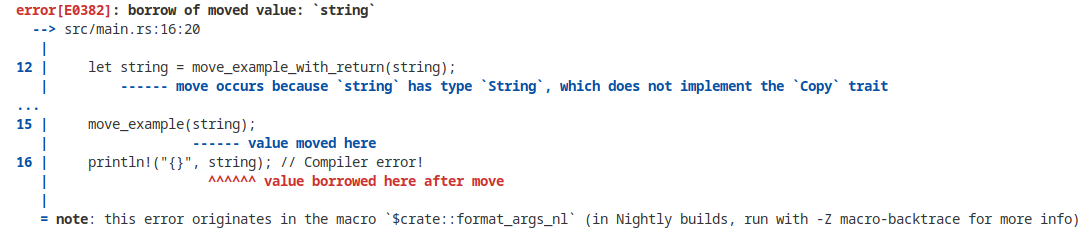
\includegraphics[scale=0.55]{kuvat/move_error_light.png}}
  \caption{Resurssin käyttöyritys siirron jälkeen johtaa käännösvirheeseen.}
  \label{rust_move_image}
\end{figure}

Omistajuuden siirtymisen voi välttää käyttämällä viittauksia (engl. reference) resursseihin. Viittaukset ovat oletuksena muuttumattomia, mutta Rustissa on myös mahdollista tehdä viittauksia, jonka kautta arvoa voi muokata~\cite[p.~147]{10.1145/3418295}. Rustin kääntäjän lainausten tarkistaja (engl. borrow checker) tarkistaa, että resurssiin on kulloinkin olemassa vain joko muuttumattomia viittauksia tai tasan yksi muokattavissa oleva viittaus~\cite[chapter~4.2]{rustbook}. Samaan resurssiin ei voi olla samanaikaisesti olemassa muuttumattomia ja muokattavissa olevia viittauksia. Viittausten rajoittaminen tällä tavalla estää kilpailutilanteiden synnyn, vaikka resurssia muokattaisiinkin viittauksen kautta. Ohjelmoija voi olla varma, että muuttumattoman viittauksen osoittama arvo ei voi muuttua, niin kauan kun viittaus on olemassa~\cite[chapter~4.2]{rustbook}. Viittauksilla resurssin voi antaa argumenttina funktiolle ja jatkaa sen käyttöä myöhemmin, ilman että funktion tulee palauttaa resurssin omistajuutta.

Rustissa jokaisella viittauksella on elinaika (engl. lifetime), jonka tarkoitus on varmistaa, että viittaukset ovat olemassa niin kauan kuin niitä tarvitaan. Kääntäjä osaa usein päätellä elinajan automaattisesti, mutta joskus ohjelmoijan täytyy itse kertoa kääntäjällä viittauksen elinaika. Elinajan merkintä kertoo kääntäjälle, että kaikki saman elinajan omaavat viittaukset ovat voimassa vähintään elinajan verran. Elinajasta Rustissa huolehtii lainausten tarkistaja, joka vertaa elinaikoja keskenään ja tarkistaa viittausten voimassaolon. Elinajan ja lainaustarkistajan ansiosta roikkuvaa osoitinta (engl. dangling pointer) eli osoitinta, jonka osoittama muistialue on siirtynyt toisen osoittimen käyttöön, ei voi syntyä. Rustissa on myös erityinen elinaika \textit{'static}, joka tarkoittaa viittauksen olevan voimassa koko ohjelman elinajan.~\cite[chapter~10.3]{rustbook}

Ohjelmalistaus \ref{lifetime_rust} ja kuva \ref{lifetime_error_rust} esittelevät elinajan ilmoittamisen eksplisiittisesti ja kääntäjän antaman virheen, mikäli se ei osaa päätellä elinaikaa. Elinajan ilmoittaminen on pakollista listauksessa, koska kääntäjä ei tiedä käännösvaiheessa, onko funktiosta palautuva viittaus \textit{str1} vai \textit{str2}, jolloin kääntäjälle tulee ilmoittaa, että molemmat ovat olemassa yhtä kauan kuin palautettava viittaus.

\begin{minipage}{\linewidth}
\lstinputlisting[language=rust, caption=Elinajan ilmoittaminen Rustissa., label={lifetime_rust}]{koodiesimerkit/lifetimes.rs}
\end{minipage}

\begin{figure}[h]
  \frame{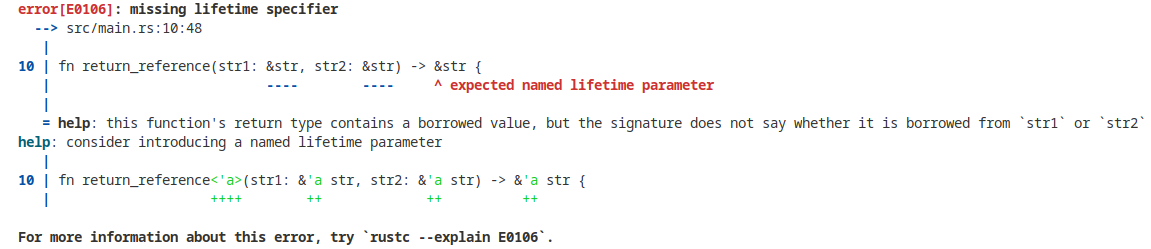
\includegraphics[scale=0.55]{kuvat/lifetime_error_light.png}}
  \caption{Kääntäjä ei osaa päätellä elinaikaa, joten sen poisjättäminen johtaisi virheeseen.}
  \label{lifetime_error_rust}
\end{figure}

\section{Säikeet}
Rust mahdollistaa säikeiden käytön tarjoamalla rajapinnan, jonka kautta säikeiden käyttäminen on turvallista. Rustin omistajuusjärjestelmä takaa, että resurssin omistajuus on yhdellä säikeellä, jolloin moni säie ei voi muokata samaa resurssia. Näin voidaan välttää kilpailutilanteet montaakin säiettä käytettäessä~\cite[chapter~16]{rustbook}. 

Rust myös mahdollistaa tilan jakamisen ja omistajuuden siirtämisen säikeiden välillä käyttämällä viestintäkanavia, joiden avulla resurssi ja sen omistajuus voidaan siirtää säikeeltä toiselle~\cite[chapter~16.2]{rustbook}. Kanavien lisäksi säikeet voivat jakaa tilan hyödyntämällä lukkiutuvia tyyppejä kuten Mutex- ja Arc-tyyppejä. Rustin kääntäjä varmistaa, että jaettuja resursseja käytetään säieturvallisesti älykkäiden osoittimien kautta~\cite[chapter~16.3]{rustbook}. Ohjelmalistaus \ref{rust_thread} esittelee jaetun resurssin käyttöä säikeissä Rustissa.


\begin{minipage}{\linewidth}
\lstinputlisting[language=rust, caption=Tilan jakaminen säikeissä Arc- ja Mutex-tyyppien avulla., label={rust_thread}]{koodiesimerkit/threads.rs}
\end{minipage}

\section{Cargo-pakettihallinta}
Rust sisältää kappaleessa \ref{kirjastot} mainitun Cargo-nimisen pakettihallintaohjelman, joka mahdollistaa kirjastojen sisällyttämisen ohjelmaan helposti. Cargon avulla projektin riippuvuuksia voidaan päivittää tai niiden versiota alentaa, jolloin kirjastojen aiheuttamia ongelmia on helppo paikata esimerkiksi tilanteessa, jossa kirjaston ylläpitäjä paikkaa löydetyn haavoittuvuuden ja päivitys halutaan mahdollisimman nopeasti sisällyttää kirjastoa käyttävään ohjelmaan. Cargolla voi asentaa riippuvuuksia crates io-rekisteristä, versionhallintapalveluista tai paikallisesti. Kirjastot ja niiden versiot määritetään Cargo.toml-tiedostoon käyttäen Semver-syntaksia, jolla voidaan määrittää sallitut versionumerot kirjastoille. Cargo luo Cargo.lock tiedoston, jossa on kyseisen ohjelman käyttämät kirjastot ja niiden käytössä olevat versiot. Kirjastot voi päivittää \textit{cargo update}-komennolla, jolloin kaikki kirjastot päivittyvät korkeimpaan Cargo.toml tiedostossa sallittuun versioon.

\section{Rustin heikkoudet}
Rustin turvajärjestelmät eivät pysty ratkaisemaan kaikkia C-kielien haasteita eivätkä ne myöskään estä ohjelmoijaa tekemästä virheitä. Esimerkiksi muistivuoto on mahdollista Rustissa luomalla kiertävä viittaus (engl. cyclic reference), jossa toisiinsa viittaavat indeksit aiheuttavat sen, että indeksille varattua muistia ei koskaan vapauteta~\cite[chapter~15.6]{rustbook}. Rustissa kiertävän viittauksen luoma ongelma voidaan ratkaista käyttämällä heikkoa viittausta Weak<T>-osoittimen avulla. Heikko viittaus ei estä resurssin pudottamista, minkä johdosta toisiinsa viittaavat indeksit pudotetaan samaan aikaan niiden osoittimien kanssa. Kuva \ref{cyclic_reference} havainnollistaa kiertävän viittauksen luomaa muistivuotoa.

\begin{figure}[H]
  \frame{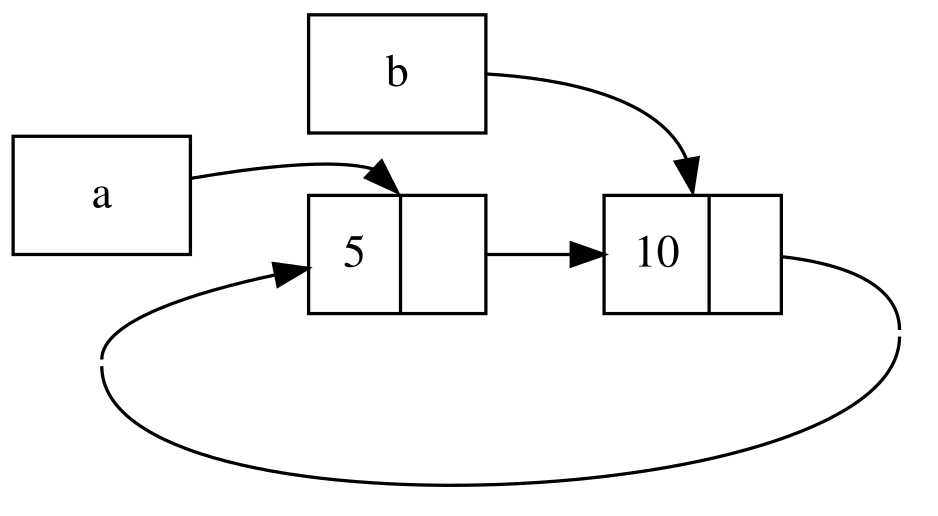
\includegraphics[scale=0.55]{kuvat/cyclic.png}}
  \caption{Kiertävässä viittauksessa muistia ei vapauteta, vaikka a ja b pudotetaan, sillä niiden osoittamat indeksit viittaavat toisiinsa~\cite[chapter~15.6]{rustbook}.}
  \label{cyclic_reference}
\end{figure}

Muistivuodon lisäksi säikeiden lukkiutumistilanne on mahdollinen ongelma Rustissa, sillä mikään Rustin turvajärjestelmistä ei estä tilannetta, jossa säikeet odottavat toistensa käyttämän resurssin vapautumista. Rustin turvajärjestelmät voivat johtaa lisäksi pitempään kehitysaikaan, minkä johdosta se ei välttämättä sovellu kovin hyvin konseptin todennukseen (engl. proof of concept) tai muihin lyhyisiin projekteihin, joissa koodin oikeellisuus ja kaikkien virhetilanteiden huomioiminen ei ole oleellista. 

Rustin opettelu voi myös viedä paljon aikaa, jolloin sen käyttöönotto ei välttämättä suju kovin helposti. Tästä johtuen Rustin käyttöönoton perustelu voi olla haastavaa esimerkiksi yritysmaailmassa. Lisäksi Rust-kielen osaajia voi olla vaikea löytää, jolloin voi syntyä tilanne, jossa Rustia ei nähdä järkevänä opetella, koska sille ei löydy työpaikkoja, eikä Rustia oteta käyttöön, koska sillä ei ole tarpeeksi osaajia. Rustin viralliset sivut tarjoavat kuitenkin paljon opetusmateriaalia eri tasoisille kielen osaajille, mikä helpottaa opettelua.

Rustin ekosysteemi on vielä nuori, joten on mahdollista, että jollekin kehittäjän haluamalle toiminnallisuudelle tai integraatiolle ei ole vielä valmista kirjastoa tai kirjasto ei ole vielä vakaa, jolloin kehittäjän täytyy joko kirjoittaa oma kirjasto tai turvautua toisella kielellä tehtyyn integraatioon, jolloin Rustin tarjoamat turvaominaisuudet menetetään kyseisen toiminnallisuuden osalta. Rust kuitenkin mahdollistaa tämän FFI:n eli Foreign Function Interfacen kautta, jonka avulla voidaan kutsua toisella kielellä kirjoitettuja funktioita.

Tiettyjen tietorakenteiden toteuttaminen Rustissa voi osoittautua turvaominaisuuksien takia hankalaksi, mikä puolestaan voi johtaa unsafe-tilan suosimiseen, jossa osa kääntäjän turvallisuusominaisuuksista kytketään pois päältä~\cite[chapter~19.1]{rustbook}. Tutkimus kehittäjien unsafe-tilan käyttöön havaitsi, että suurin osa crates.io:sta löytyvistä kirjastoista käyttää unsafe-tilaa jossakin muodossa, mutta suurimassa osassa se on abstraktoitu turvallisen rajapinnan taakse, jolloin kirjaston käyttäjän ei tarvitse käyttää unsafe-tilaa omassa koodissaan~\cite[p.~252]{unsafe}. Unsafe-tilan käyttö saattaa olla tietyissä matalan tason operaatioissa pakollista, mutta suurimmassa osassa ohjelmia sen käyttö on tarpeetonta. Unsafe tila ei myöskään poista lainauksen tarkistajaa ja omistajuutta käytöstä vaan se vaikuttaa vain muistiturvallisuustakuisiin~\cite[chapter~19.1]{rustbook}.\chapter{Loppupäätelmät} \label{Loppupäätelmät}

Tutkielma osoittaa, että Rust on ominaisuuksiltaan käytettävissä samanlaisissa sovelluksissa C-kielien kanssa. Lisäksi Rustin käytöllä voidaan poistaa monia vakavien haavoittuvuuksien ja ohjelmien epävakauden aiheuttajia. Rustin ominaisuudet voivat myös helpottaa kehitystyötä tarjoamalla helpon riippuvuuksienhallinnan sekä hyvät virheenjäljitystyökalut. Rust ei kuitenkaan poistaa vastuuta ohjelmoijalta kokonaan eikä estä ohjelmoijaa tekemästä virheitä, jotka vaikuttavat ohjelman turvallisuuteen ja vakauteen. Tästä huolimatta Rustin käytöllä saavutetut hyödyt ovat riittäviä, jotta sen käyttö C-kielien sijaan on perusteltua, mikäli jokin syy ei estä sen käyttöä.

Rustin käyttöönoton suurimmat haasteet ovat ekosysteemin nuoruus sekä osaamisen vähäisyys verrattuna C-kieliin. Tätä puutetta paikkaa kieleen vahvasti sidoksissa oleva pakettihallintaratkaisu kolmannen osapuolten kirjastoja ja riippuvuuksia varten sekä helposti saatavilla oleva ja kattava dokumentaatio ja opetusmateriaali. Rustin käyttöönottoa edesauttaa myös se, että sillä on useiden suurien yritysten tuki. Rustin kehityksen vastuu siirtyikin vuonna 2021 Mozillalta Rust Foundation-järjestölle, jonka perustajina ovat AWS, Huawei, Google, Microsoft ja Mozilla~\cite{rustfoundation}.

Tutkielman aihetta käsiteltiin vahvasti Rustin hyötyjen näkökulmasta, jolloin sen haasteet jäivät vähemmälle huomiolle. Samoin C-kieliä käsiteltiin niiden aiheuttamien haasteiden kautta, jolloin niihin vuosien aikana tehdyt turvallisuutta ja vakautta parantavat lisäykset jäivät vähemmälle huomiolle. Rustin käyttö ei ole ongelmatonta ja sen käytön yleistyessä ilmenee varmasti sille ominaisia ongelmia. Rustin haasteista ja sen ominaisuuksiin liittyvistä ongelmista olisi mahdollista tehdä jatkotutkimuksia. Lisäksi C-kielille kehitetyistä muistiturvallisuutta parantavista sovelluksista ja ohjelmointitekniikoista olisi mahdollista tehdä syvällisempiä jatkotutkimuksia. Myös Rustin vaikutuksista kehitysajan pituuteen voisi tehdä tutkimuksia, sillä se on yleinen kritiikki Rustia kohtaan.

Tutkielma esittää, että Rust olisi mahdollinen korvaaja C-kielille, mutta tämä ei tarkoita, että kaikki olemassa oleva C-kielillä kirjoitettu koodi pitäisi uudelleenkirjoittaa Rustilla. Sen sijaan Rustia tulisi harkita C-kielille vaihtoehtona uusia projekteja aloitettaessa, sekä silloin, kun lisätään ominaisuuksia C:llä tai \Cpp:lla kirjoitettuun ohjelmaan. Rust tarjoaa työkalut, joilla on mahdollista rakentaa uutta toiminnallisuutta C-kielillä kirjoitetun koodin päälle, mikä nähdään esimerkiksi Linux-ytimessä, jossa Rust on tarkoitus ottaa käyttöön toisena sallittuna kehityskielenä.

%\input{file_name_of_chapter_x}
%\input{file_name_of_chapter_y}

% The thesis main content ends here.

\printbibliography

\begin{comment}
Important! Create the appendix chapters with command \textbackslash appchapter\{some
name\} instead of \textbackslash chapter\{some name\} for the automagic
page counting to work!
\end{comment}

\end{document}
